\chapter{Strategie und Taktik}
\label{sec:module.StrategieTaktik}


\section{Influence Map}
\label{sec:module.InfluenceMap}
\begin{figure}[H]
\centering
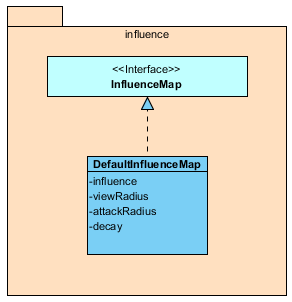
\includegraphics[width=0.5\textwidth]{91_bilder/strategyInfluence}
\caption{Influence Map Klassendiagramm}
\label{fig.strategyInfluence}
\end{figure}

Die Influence Map haben wir nach den Beschreibungen im Buch \cite{ARTIFICIALINTELLIGENCEFORGAMES} implementiert. Jede bekannte Spieleinheit auf der Spielkarte 'strahlt' eine gewissen Einfluss aus. In unserer Implementation unterscheiden wir zwischen drei Einflussradien, der Angriffsradius, der erweiterte Angriffsradius und der Sichtradius. Den Radien haben wir folgende Werte zugewiesen. 


\begin{tabular}{p{5cm}|p{3cm}|p{3cm}}
 Radius & Wert & Radius in Tiles* \\
 Angriffsradius & 50 & 2.2 \\
 Erweiterter Angriffsradius & 30 & 5  \\
 Sichtradius & 10 & 8.8 \\
 \end{tabular}
 
 * Die Radiusl�nge kann je nach Spieleinstellung �ndern. Angegeben sind die Defaultwerte.

Wir verenden die Influence Map vorallem f�r die Bestimmung der Sicherheit. Abgebildet ist eine Sicherheitskarte (Desirability Map) f�r den orangen Spieler, wobei die Einflusswerte des Gegners von den Einflusswerten des eigenen Spielers je Tile subtrahiert werden. Positive Werte bedeuten sicheres Terrain und negative Werte unsicheres, vom Gegner kontrolliertes Gebiet.

\begin{figure}[H]
\centering
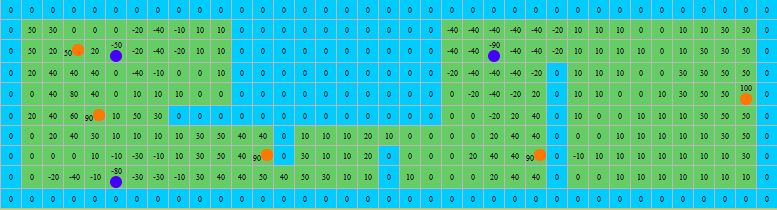
\includegraphics[width=0.99\textwidth]{91_bilder/influence01.jpg}
\caption{Influence Map, dargestellt ist die Sicherheit je Tile.}
\label{fig.InfluenceMap01}
\end{figure}

\subsection{Update}
\label{subsec:module.InfluenceMap.Update}

Die Influence Map wird zu Beginn des Spiels initialisiert, danach wird vor jeder Spielrunde ein Update gemacht. Dabei definert ein Decay-Wert zwischen 0 und 1, wieviel von den alten Werten beibehalten wird. Folgende Formel bestimmt den neuen Wert f�r jede Zelle:


\(val_{(x,y)} = val_{(x,y)} * decay + newval_{(x,y)} * (1-decay)\)


\subsection{Andwendungsf�lle}
\label{subsec:module.InfluenceMap.Andwendungsf�lle}

In folgenden Modulen ber�cksichtigen wir Werte aus Influence Map um Entscheide zu f�llen.

\begin{itemize}
\item
\textbf{Pfadsuche mit Influence Map Ber�cksichtigung}: Siehe Kapitel \ref{subsec:module.Suchalgorithmen.Pfadsuche.WithInfluenceMap}
\item
\textbf{CombatSituation: Flucht}: M�ssen wir die Flucht ergreifen, bewegen wir unsere Ameise auf das n�chste sicherste Tile.
\item
\textbf{Abbruch Mission}: Falls eine Ameise auf einer andere Mission als die GatherFoodMission ist und ein Food Tile in seiner N�he antrifft, wird abgewogen ob die Mission zu Gunsten von Futter sammeln abgebrochen werden soll. Dabei ist ein Entscheidungsfaktor auch die 'Sicherheit' des Futters. Falls das Futter nicht auf einem sicheren Weg geholt werden kann, wird die Mission nicht abgebrochen.
\end{itemize}

Nat�rlich k�nnte man die Influence Map auch f�r weitere Entscheidungen verwenden. Auch der Einsatz von Spannungskarte (Tension Map), welche auch auf der InfluenceMap aufbaut, w�re denkbar. Dies wurde w�hrend dieser Arbeit nicht angeschaut bzw. implementiert.


\section{Combat Situations}
\label{sec:module.CombatSituation}

Kampfsiuationen werden immer dann erstellt wenn gegnerische Ameisen auf unsere Ameisen treffen. Dies ist vorallem der Fall wenn ein gegnerischer H�gel angegriffen wird, oder unserer H�gel verteidigt werden muss. Eine Kampfsituation kann sich aber auch sonst wo auf der Karte ereignen.

\subsection{DefaultCombatPositioning}
\label{sec:module.CombatSituation.DefaultCombatPositioning}

DefaultCombatPositioning implementiert das Interface CombatPositioning und f�hrt die Postionierung f�r die drei Verhalten FLEE, DEFEND, ATTACK an. Das Verhalten wird in der Methode determineMode(...) wie folgt bestimmt, wobei das 'DEFAULT' Verhalten dem ATTACK-Verhalten entspricht.

\begin{verbatim}
protected Mode determineMode() {
    final boolean enemyIsSuperior = enemyUnits.size() > myUnits.size();
    if (enemyIsSuperior)
        return Mode.FLEE;
    return Mode.DEFAULT;
}
\end{verbatim}

Wird nicht ein DefaultCombatPositioning initialisiert, sondern ein AttackingCombatPositioning (in der AttackHillMission) oder ein DefendingCombatPositioning (in der DefendHillMission) so wird das Verhalten anders bestimmt, indem die Methode determineMode() �berschrieben ist.

TODO DIAGRAMM

\textbf{DefendingCombatPositioning}

TODO

\textbf{AttackingCombatPositioning}

TODO

Die bereits erw�hnten Verhalten, nehmen folgende Positionierung der Ameisen vor.

\subsubsection{FLEE}
\label{sec:module.CombatSituation.DefaultCombatPositioning.Flee}

F�r jede Unit wird das sicherste Nachbartile mittels Influence Map bestimmt. Die Unit verschieb sich auf das sicherste Nachbartile.

\begin{verbatim}
for (Tile myUnit : myUnits) {
    nextMoves.put(myUnit, map.getSafestNeighbour(myUnit, influenceMap));
}
\end{verbatim}

\subsubsection{DEFEND}
\label{sec:module.CombatSituation.DefaultCombatPositioning.Defend}

TODO

\subsubsection{ATTACK}
\label{sec:module.CombatSituation.DefaultCombatPositioning.Attack}

TODO